\chapter[المتغير العشوائي]{المتغير العشوائي \\ \en{Random Variable}}

\section{التعريف}
المتغير العشوائي \(X\) هو فكرة تربط فضاء العينة بالاعداد الحقيقية. حيث اذا كان لدينا تجربة عشوائية ما فإن المتغير العشوائي سوف يربط كل عنصر من فضاء العينة بعدد حقيقي

\begin{example}
	\begin{english}
			\en{Consider the experiment of tossing a coin twice, then}
	\end{english}
	
	\noindent
	تجربة قلب عملة معدنية مرتين فضاء العينة فيها
	\[
	\Omega = \{TT, TH, HT, HH\}
	\]
\end{example}
\begin{english}
	Let \(X\) be the r.v. denote the number of heads
\end{english}

\noindent 
	هنا فرضنا ان \(X\) هو المتغير العشوائي الذي يمثل عدد الوجوه التي تظهر \(H\)، أي أن 
	\[
	X(w) = \begin{cases}
		0 & \text{if}\quad w = TT\\
		1 & \text{if}\quad  w = TH, HT\\
		2 & \text{if}\quad  w = HH
	\end{cases}
	\]
 	اذن فضاء المتغير \(X\) هو \(\mathcal{A} = \{0,1,2\}\)
 	\begin{english}
 		\begin{figure}[ht]
 			\centering
 				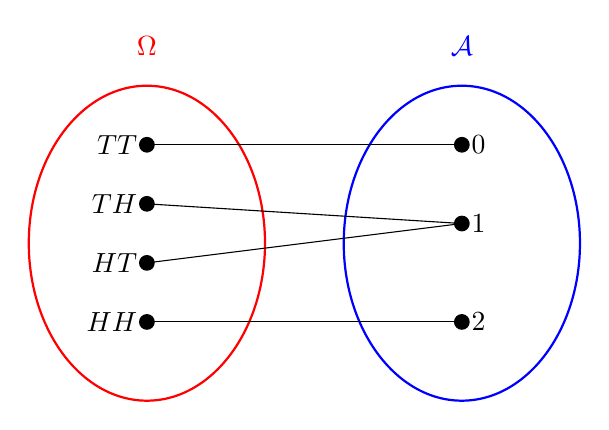
\begin{tikzpicture}
 				\draw[thick, color=red] (0,0) ellipse[x radius=1.5, y radius=2] +(0, 2.5) node{$\Omega$};
 				\draw[thick, color=blue] (4,0) ellipse[x radius=1.5, y radius=2] +(0, 2.5) node{$\mathcal{A}$};
 				\coordinate (tt) at (0,1.25);
 				\coordinate (th) at (0,0.5);
 				\coordinate (ht) at (0,-0.25);
 				\coordinate (hh) at (0,-1);
 				
 				\coordinate (0) at (4,1.25);
 				\coordinate (1) at (4,0.25);
 				\coordinate (2) at (4,-1);
 				
 				\fill (tt) circle[radius=0.1] node[left]{$TT$}; 
 				\fill (th) circle[radius=0.1] node[left]{$TH$}; 
 				\fill (ht) circle[radius=0.1] node[left]{$HT$}; 
 				\fill (hh) circle[radius=0.1] node[left]{$HH$}; 
 				
 				\fill (0) circle[radius=0.1] node[right]{$0$};
 				\fill (1) circle[radius=0.1] node[right]{$1$};
 				\fill (2) circle[radius=0.1] node[right]{$2$};
 				
 				\draw[-] (tt) to (0);
 				\draw[-] (th) to (1);
 				\draw[-] (ht) to (1);
 				\draw[-] (hh) to (2); 			
 			\end{tikzpicture}
 		\end{figure}
 	\end{english}
 	
 	\begin{note}
 		هناك نوعان رئيسيان للمتغير العشوائي
        \begin{enumerate}[label=\textbf{\arabic*}.]
 			\item \textbf{النوع المستمر \en{Continous type}:} هو المتغير الذي يأخذ قيم بين عددين (فترة) مثل  \(1<X<3\)
 			\item \textbf{النوع المتقطع \en{Discrete type}:} هو المتغير الذي يأخذ قيم معدودة مثل \\ \(X=0,1,2,3,\dots\)
 		\end{enumerate}
 	\end{note}
 	
\section[الدالة الاحتمالية]{الدالة الاحتمالية \en{Probability Function (\textit{p.f.})}}
الدالة الاحتمالية هي تمثل الاحتمالية للمتغير العشوائي $X$ الذي يأخذ قيم حقيقية من فضاء العينة. و هناك نوعان من الدالة الاحتمالية:
 	
\subsection*{1. دالة الكتلة الاحتمالية \en{Probability Mass Function (\textit{p.m.f.})}}
عندما يكون $X$ متغير عشوائي متقطع و يأخذ القيم $x_1, x_2, \dots, x_n$ فإن الدالة الاحتمالية تعرف بالشكل
\[
f(x) = P_r(x) = \begin{cases}
	P_r(X=x_i) & i = 1,2,\dots,n \\
	o & \text{otherwise}
\end{cases}
\]
مع الخصائص الآتية 
\begin{enumerate}
	\item $P_r(x_i) \geq 0$ لكل $i=1,2,\dots,n$ اي بمعنى ان الدالة غير سالبة.
	\item $\sum_i P_r(x_i) = 1$.
	\item $P_r(x\in A) = \sum_{x\in A} P_r(x)$. حيث ان $A$ مجموعة جزئية من $X$.
\end{enumerate}

\begin{example}
	\begin{english}
		Let \(X\) be a random variable of discrete type with
		\[
		f(x) = \begin{cases}
			\dfrac{x}{15} & x=1,2,3,4,5 \\
			0 & \text{otherwise}
		\end{cases} 
		\]
		\begin{enumerate}
			\item Is \(f(x)\) a \textit{p.m.f.}
			\item If \(A=\{2,3\}\) find \(P(A)\)
		\end{enumerate}
	\end{english}
	\noindent
	المطلب الاول هو هل ان الدالة المعطاة تمثل دالة احتمالية ام لا و المطلب الثاني ايجاد احتمالية المجموعة \(A\).
\end{example}
\noindent
\textbf{الحل}
	\begin{enumerate}[topsep=0pt]
		\item  يجب ان نطبق الشرطان. الاول ان الدالة غير سالبة اي نجد قيم الدالة عند المجال ونرى
		\[
		f(1) = \frac{1}{15}, f(2) = \frac{2}{15}, f(3)=\frac{3}{15}, f(4)=\frac{4}{15}, f(5)=\frac{5}{15}
		\]
		\[
		f(x) = 0, \text{otherwise}
		\]
		اذن $f(x)\geq0$. الآن نجد مجموع الدالة لكل قيم المجال و يجب ان يكون الناتج 1:
		\begin{align*}
			\sum_x f(x) &= \sum_x \frac{x}{15}\\
			&= \frac{1}{15} + \frac{2}{15} + \frac{3}{15} + \frac{4}{15} + \frac{5}{15}\\
			&= \frac{15}{15} = 1
		\end{align*}
		اذن الدالة $f(x)$ هي دالة كتلة احتمالية \hspace{10pt}
		\en{
			$\therefore f(x)$ is \textit{p.m.f}
		}
		
		\item لنجد احتمالية المجموعة \(A\) نجد مجموع الدالة على عناصر \(A\).
		\begin{align*}
			P(A) &= \sum_{x\in A} P_r(x)\\
			&= P_r(X=2) + P_r(X=3)\\
			&= \frac{2}{15}+\frac{3}{15}\\
			&= \frac{5}{15} = \frac{1}{3}
		\end{align*}
	\end{enumerate}

\subsection*{2- دالة الكثافة الاحتمالية \en{Probability Density Function \textit{p.d.f.}}}
عندما يكون $X$ متغير عشوائي مستمر أي يأخذ قيم بين عددين $x_1<X<x_2$. اذن $f(x)$ هي \en{\textit{p.d.f.}} و تمتلك الخواص الآتية:
\begin{enumerate}
	\item \(f(x) \geq 0\)
	\item \(\displaystyle \int_{\forall x}f(x) \, dx = 1\)
	\item \(\displaystyle P_r(a<X<b) = \int_a^b f(x)\, dx\)
\end{enumerate}

\begin{example}
	\begin{english}
		Let $X$ be r.v. of continuous type with
		\[
		f(x) = \begin{cases}
			e^{-x} & x> 0 \\
			0 & \text{otherwise}
		\end{cases}
		\]
		Is $f(x)$ \textit{p.d.f.} of $X$? graph $f(x)$
	\end{english}
	
	\noindent
	لدينا متغير عشوائي مستمر مع الدالة $f(x)$ هل أن الدالة تمثل دالة كتلة احتمالية؟ مع رسم الدالة.
\end{example}
\begin{solution}
	نبطق التكامل 
	\[
	\int_{\forall x} f(x) \, dx = \int_0^\infty e^{-x} \, dx  = - [e^{-x}]^\infty_0 = - [0-1] = 1
	\]
	اذن الدالة تمثل دالة كتلة احتمالية.
			\begin{figure}[H]
			\centering
			\begin{tikzpicture}
			\begin{axis}[
				axis lines=middle,
				domain=0:5,
				xlabel={$x$},
				ylabel={$f(x)$},
				xtick={0},
				ytick={1},
				enlargelimits=true,
				samples=100,
				]
				\addplot [name path=A,domain=0:5,samples=1000] {exp(-x)};
				
				\addplot [name path=B] {0};
				
				\addplot[blue, opacity=0.3] fill between [of=A and B];
				
				\node[above left] at (0,0) {$0$};
			\end{axis}
		\end{tikzpicture}
		\end{figure}
\end{solution}

\begin{example}
	\begin{english}
		Let
		\[
		f(x) = \begin{cases}
			cx^2 & 0<x<1 \\
			0 & o.w.
		\end{cases}
		\]
		be the \textit{p.d.f.} of $X$.
		\begin{tasks}(1)
			\task Find the value of $c$
			\task Compute $P(X<\frac{1}{2})$
			\task Compute $P(X>\frac{1}{2})$
		\end{tasks}
	\end{english}
	
	\noindent
	المعطيات: دالة كتلة احتمالية (اي تحقق الشروط) و المطلوب ايجاد قيمة المجهول $c$ و بعد ذلك ايجاد الاحتماليات
\end{example}

\begin{solution}
	1) بما أن الدالة تحقق الشروط اذن تكاملها على المجال = 1 و بالتالي:
\begin{gather*}
	\therefore\int_{\forall x} f(x) \, dx = 1\\
	\Rightarrow \int_0^1 cx^2 \, dx = 1\Rightarrow c\left[\frac{x^3}{3}\right]^1_0 =1 \Rightarrow c\left[\frac{1}{3} -0 \right]=1\\
	\Rightarrow \frac{1}{3}c=1\Rightarrow \boxed{c=3}\\
	\therefore f(x) = \begin{cases}
		3x^2 & 0<x<1 \\
		0 & o.w.
	\end{cases}
\end{gather*}
2) هنا الاحتمالية اقل اي حدود التكامل من اقل قيمة في المجال (هي 0) الى الحد $\frac{1}{2}$
\[
P\left(X<\frac{1}{2}\right) = \int_0^{1/2} 3x^2 \, dx = 3 \left[\frac{x^3}{3}\right]^{1/2}_0 = \frac{1}{8}
 \]
 3) هنا الاحتمالية اكبر اي حدود التكامل من الحد الادنى $\frac{1}{2}$ الى اعلى قيمة في المجال وهي 1
 \[
P\left(X>\frac{1}{2}\right) = \int_{1/2}^1 3x^2 \, dx = 3 \left[\frac{x^3}{3}\right]^1_{1/2} = 1-\frac{1}{8} = \frac{7}{8}
 \]
\end{solution}



